\documentclass[a4paper,12pt,oneside,openany]{jsbook}

\usepackage[papersize={210truemm, 297truemm}]{geometry}
\geometry{top=40truemm,bottom=35truemm,left=25truemm,right=25truemm}
%
\usepackage[utf8]{inputenc}
\usepackage{booktabs}
\usepackage{url}
\usepackage{nidanfloat}
\usepackage{afterpage}
\usepackage{setspace}
\usepackage{multirow}
\usepackage{here}

\usepackage{amsmath,amssymb}
\usepackage{bm}
%\usepackage{graphicx}
\usepackage[dvipdfmx]{graphicx}
\usepackage{subfigure}
\usepackage{verbatim}
\usepackage{wrapfig}
\usepackage{ascmac}
\usepackage{makeidx}

\usepackage{algorithm}
\usepackage{algorithmic}
%
\setcounter{tocdepth}{3}
%
\makeindex
%余白設定
\setlength{\textwidth}{\fullwidth}
\setlength{\textheight}{35\baselineskip}
\addtolength{\textheight}{\topskip}
\setlength{\voffset}{-0.55in}
\setlength{\abovedisplayskip}{2.5pt} % 上部のマージン
\setlength{\belowdisplayskip}{2pt} % 下部のマージン
%
\newcommand{\etal}{\textit{et al}.,}
\newcommand{\ie}{\textit{i}.\textit{e}.,}
\newcommand{\eg}{\textit{e}.\textit{g}.,}
\newcommand{\reffig}[1]{図\ref{#1}}
\newcommand{\reftab}[1]{表\ref{#1}}
\newcommand{\refequ}[1]{式\ref{#1}}
\newcommand{\refsec}[1]{\ref{#1}節}

%%%%%%%%%%%%%%%%%%%%%%%%%%%%%%%%%%%%%%%%%%%%%%%%%%%%%%
%\title{タイトル}
%\author{氏名}
%\date{\today}
\begin{document}
%
%\maketitle
%
\frontmatter
%表紙
\begin{titlepage}
  \vspace*{7mm}
  \begin{center}
    \Large{平成31年度卒業論文}\\

    \vspace{40truemm}

    \LARGE{\textbf{画像付きフェイクニュースとジョークニュースの検出・分類に向けた機械学習モデルの検討}}\\

    \vspace{30truemm}

    \Large{電気通信大学 情報理工学部 総合情報学科}\\
    \Large{メディア情報学コース}\\

    \vspace{15truemm}

    \begin{table*}[h]
        \centering
        \hspace*{4em}
        \begin{tabular}{rcl}
            \large{学籍番号}&\large{:}&\large{1510151} \\
            \large{氏名}&\large{:}&\large{栁 裕太} \vspace{5truemm} \\
            \large{主任指導教員}&\large{:}&\large{田原 康之 准教授} \vspace{5truemm} \\
            \large{指導教員}&\large{:}&\large{大須賀 昭彦 教授} \vspace{5truemm} \\
            \large{指導教員}&\large{:}&\large{清 雄一 准教授} \vspace{5truemm} \\
            \large{提出年月日}&\large{:}&\large{平成31年2月8日(金)} \\
        \end{tabular}
    \end{table*}
  \end{center}
\end{titlepage}
%
%アブスト
\addcontentsline{toc}{chapter}{概要}

\chapter{概要}

%背景
SNSの発展によりあらゆる情報入手が容易になった反面,人を欺くために故意に作成された虚偽の情報であるフェイクニュースが社会問題になっている.
特に画像と併せて発信されたものは,テキストのみならず画像と併せた分析アプローチが有効である.
虚偽の情報としては,もう1つジョークニュースというものもある.
これは人を欺くためではなく,社会風刺や皮肉のために作られた情報という特徴がある.
しばしばこの2カテゴリが混同され,ジョークニュースが批判に晒されることがあることも問題となっている.

%既存課題
既にテキスト・画像を分析して真偽を判定する自動判別モデルが提案されている.
実際に真実・フェイクとのカテゴリ分類において優秀な成績を収めているものの,
ジョークとしての嘘情報と人を欺くための嘘情報が区別されていない.
ジョークも含めた3カテゴリ分類においても,テキストを対象とした研究はあれどテキスト・画像を分析して3カテゴリに分類する研究はない.


%提案
本研究では,正しい情報・ジョークニュース・フェイクニュースの3カテゴリを分類することで,
より画像つきフェイクニュースとジョークニュースの検出におけるテキスト・画像を併せた分類の有効性を確認することを目指した.


%実験結果
実際にSNSから収集した画像つきのデータセットを対象にカテゴリ分類を行った結果,3カテゴリでもマクロF値が約0.93と良好な結果を示した.
また,比較対象手法としてテキスト単体から・画像単体から分類する手法と比較した結果,
テキスト・画像と併せてあれば細かい手法に問わず一貫して優秀な分類成績を挙げた.

%
\tableofcontents
%
\mainmatter
%本文
% 背景[フェイクニュースの自動判別の必要性+ジョークニュースを区別する必要性]+想定環境の説明(導入との被りに注意)
\chapter{序論}
%
\section{背景}
% フェイクニュース
昨今のSNSの普及により,誰もが情報を発信・収集できるようになった.
特に最近ではテキストのみならず,画像や動画と併せて情報の発信が可能である.
一般論として,テキスト単体と比べて画像や動画と併せて発信されたマルチメディア情報の方が多くの注目を得やすい.
逆にこれを利用して,故意に情報を捏造して発信することによって人々を誤った方向へ扇動するフェイクニュースも存在する.
フェイクニュースが広まると、大規模なマイナスの影響が出る可能性があり、
場合によっては重要な公共の出来事に影響を及ぼしたり、操作したりすることさえある.
例えば2016年の米国大統領選では,2名の候補者を支持させるためのフェイクニュースが多く拡散され,
とりわけFacebook上では3700万回以上共有された\cite{allcott2017social}.

% ジョークニュース
虚偽の情報ながら,扇動ではなく皮肉や風刺を込めたジョークニュースも存在する.
有名な発信メディアとしては,英語ではthe Onion,日本語では虚構新聞が該当する.
あくまで扇動ではなく笑いを提供するためのものであり,
多くの場合それは批判の的にはなりにくい.
しかしながら,ジョークニュースはフェイクニュースと同じく限りなく真実を模した形式をとるため,
同じくSNS上で拡散されやすい傾向にある.

% 想定環境
当研究では,扇動のために故意に情報を捏造して発信された情報をフェイクニュース,
事実を発信した情報を正しいニュース,
そして風刺や皮肉を込めて発信された情報をジョークニュースとして定義する.

\section{先行研究}
% フェイクニュースのテキストによる分類
フェイクニュースに限らず,風評やwebページの信憑性を評価するモデルの構築の研究は数多く行われている.
例えば,福島らの研究\cite{福島隆寛2007web}では,webページの体裁から信頼性を評価するモデルが提案されている.
また,機械学習による分類が非常に盛んに行われている.
なかでもGranikらの研究\cite{Granik8100379}やGildaの研究\cite{Gilda8305411},そして松尾の研究\cite{松尾省吾2018master}により,
単語埋め込みとナイーブベイズ分類器やSVM,決定木といった教師あり学習を組み合わせることによって,
フェイクニュースや流言を分類するタスクで優秀な分類成果を挙げることが報告されている.
ほかにもWuらの研究\cite{wu2018tracing}によると,SNS上で拡散された情報に対して,
``誰が・どのような経緯で拡散したか''という情報から信憑性を判断するモデルも提案されている. 
Rubinらの研究\cite{rubin2016fake}によれば,正しいニュース・ジョークニュースの分類にもこのアプローチが有効であることが示されている.
正しいニュース・フェイクニュース・ジョークニュースの3カテゴリ分類においても研究が行われている.
特にHorneとSibelの研究\cite{horne2017just}によると,フェイクニュースは正しいニュースよりジョークニュースに近い性質をもち,
真実に近い形式をとるほど高い説得力をもつことが示されている.

% マルチメディアでフェイクニュース分類
上記の機械学習を使った研究では,いずれもテキストのみの情報を対象としている.
別の対象として,テキスト・画像を併せた情報を分類する機械学習モデルの検討も数多く行われている.
大まかな形としては,まずテキスト・画像を何らかの方法でベクトル化する.
その後2種のベクトルを結合し,真偽判定を行うモデルに渡す形をとっている.
例えばJinらの研究\cite{jin2017multimodal}では,テキストではLSTM,画像ではVGG-19を使用してベクトル化しており,
更にAttentionとソーシャルコンテキスト(ハッシュタグ,URL等)によって更に高精度な分類を行うモデルが提案されている.
またWangらの研究\cite{wang2018eann}では,EANNというモデルが提案されている.
これは画像のベクトル化においては同じくVGG-19を使用しているが,テキストではテキストCNNを使用している.
% このモデルの大きな特長として,敵対的生成ネットワーク(GAN)を模倣する形をとることが挙げられる.
% ニュースを学習する際には,どうしても扱うニュースが扱うイベントの偏りによる影響を受けてしまう.
% このイベントによる特殊性を排するために,真偽分類に加えて扱われたイベントも分類することによって,
% 特徴化する際にイベントによる特殊性を排するアプローチが行われている.
% 実際にこれによって分類精度が改善した点が上記研究によって報告されている.
% * GANは当研究では使わないので記述から外すことにした

\section{課題}
上記のEANNモデルのような画像・テキスト双方を扱うモデルでは,実際に真実・フェイクとのカテゴリ分類において画像単独・テキスト単独の分類に比べて優秀な成績を収めている\cite{wang2018eann}.\@
しかしながら,あくまで``真実なのかそうでないのか''という2カテゴリで分類しているため,
``他者を欺くための情報なのか,皮肉・風刺を込めた情報なのか''という観点での分析がなされていない.

% 本研究
本研究では,画像つきで発信された情報に対して,正しい情報か・フェイクニュースか・ジョークニュースかを判断するモデルを構築する.
このモデルを使い,従来から画像・テキスト複合のデータセットに対して3カテゴリでも優秀な分類が行えることを示すことを目指す.
それにより,SNSユーザの情報収集を支援するエージェントの開発につなげることが可能となる.

% 実験
上記の提案する情報分類システムを検証するために,
事前に用意されたデータセットを用いて10 分割交差検定によって分析を行う.
また上記システムの分類性能を評価するために,
画像・テキスト単独で分類を行った結果と比較することで,
提案システムが目標に適していることを示す.
その結果テキスト単独でのマクロF値が約0.22,画像単独でのマクロF値が約0.40であったのに比べ,
提案モデルのマクロF値は約0.93という数値を出し,提案モデルの有効性が示された.

% \bibliography{../ref/ref}

%
\chapter{提案手法}
%
\section{モデル概観}
この章では,提案モデルがもつ複合特徴量抽出器とニュース分類器について紹介する.
その後にこの2要素を統合して転移学習が可能な表現を学習する方法について説明する.
% 最後に,詳細なアルゴリズムフローを付加する. 
今回提案したモデルは,以下の図\ref{fig:model}の通りである.

提案モデルの目的は,画像と文章で発信された情報に対して,
正しいニュースか・フェイクニュースか・ジョークニュースかを分類するために,
必要な特徴表現を学習することであった.
提案モデルは複合特徴量抽出器とニュース分類器の大きく2部分に分けることができた.
まず複合特徴量抽出器は,今回扱う情報が文章と画像を含むため,
各メディアに対して特徴化する抽出器があった.
その後それぞれの特徴を1つに連結し,複合特徴を形成した.
複合特徴はニュース分類器に送られ,最終的には3カテゴリのどれに該当するかが判断された.
% 
\begin{figure}[H]
    \centering
    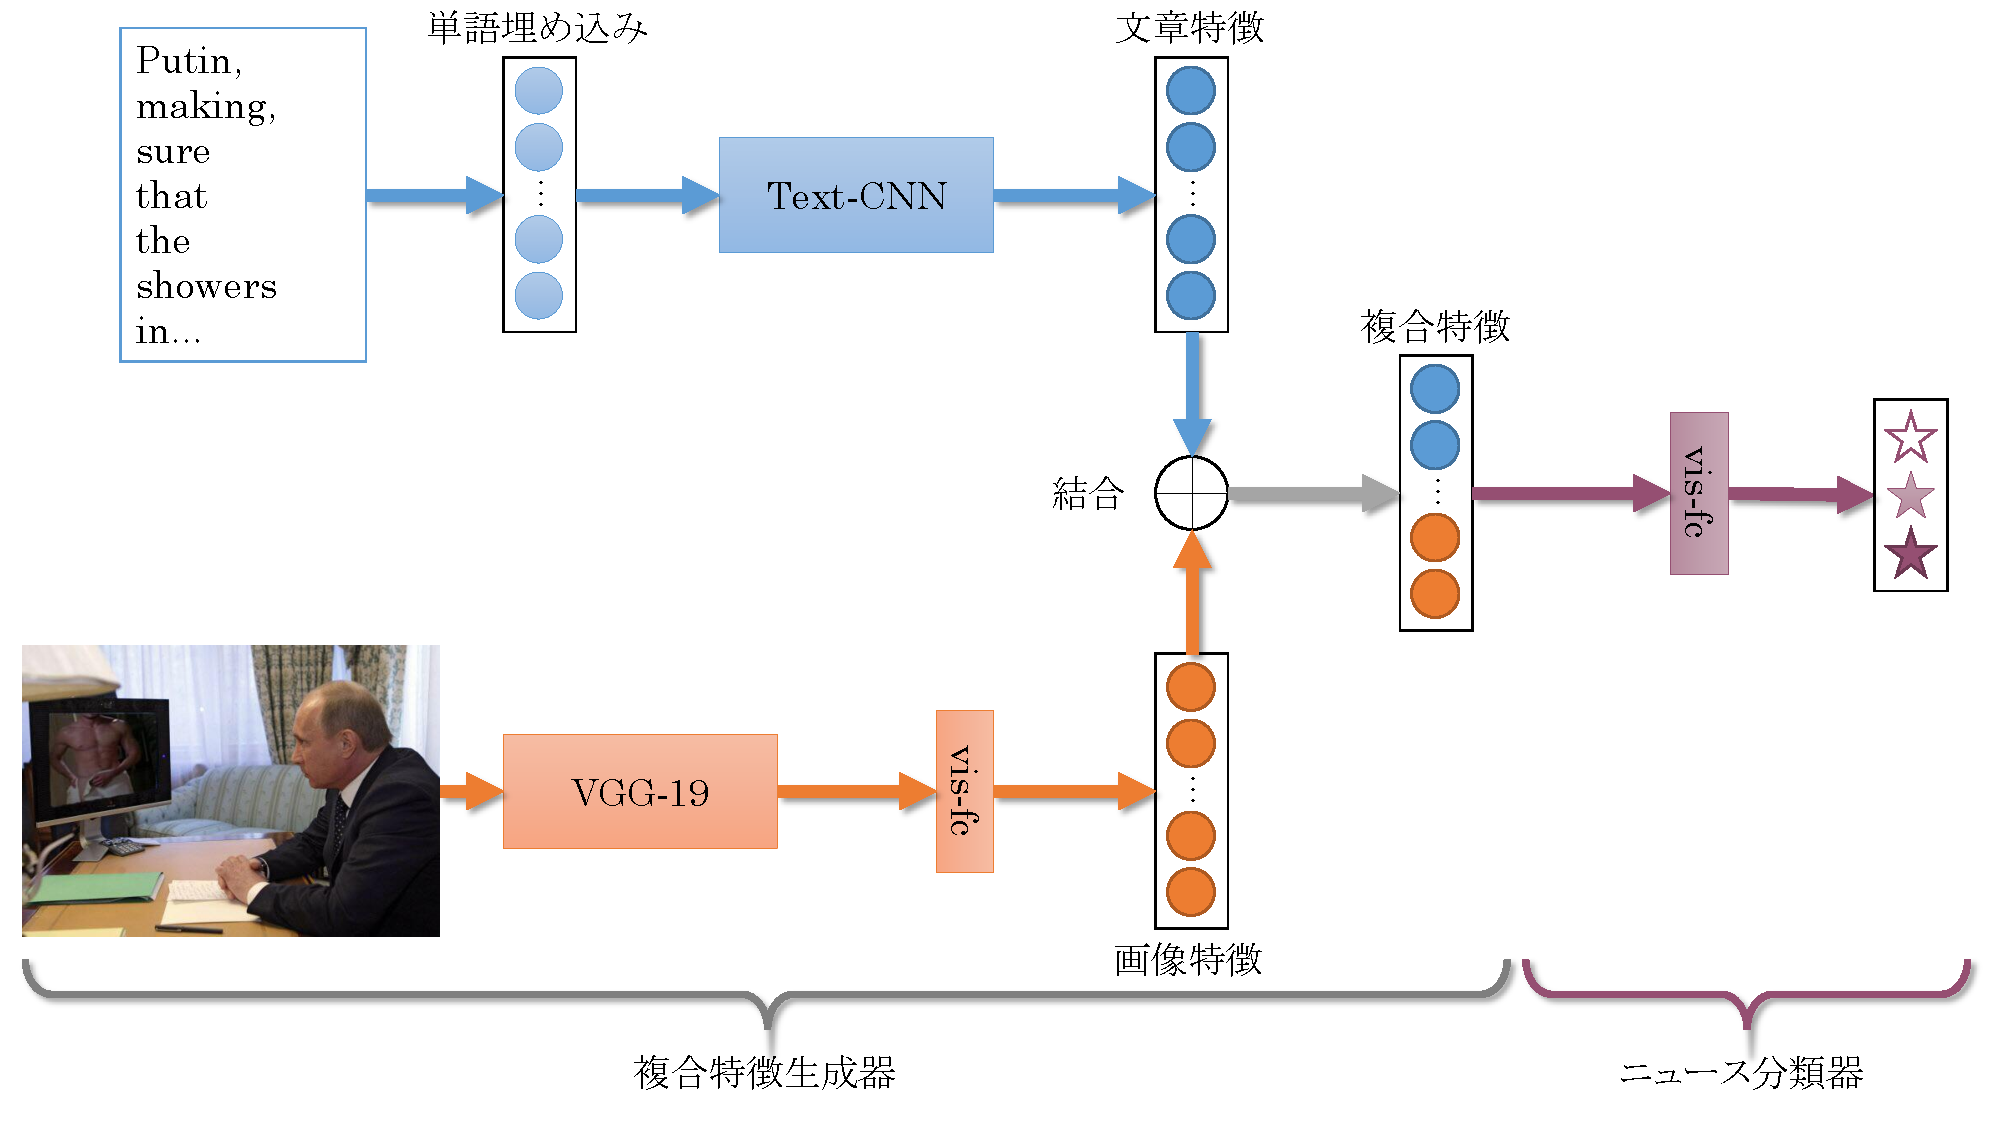
\includegraphics[width=0.8\linewidth]{images/methodology.pdf}
    \caption{提案モデル図.青: 文章特徴量抽出器,橙: 画像特徴抽出器,紫: ニュース分類器.}
    \label{fig:model}
\end{figure}
%
\section{複合特徴抽出器}
%
\subsection{文章特徴} \label{subsec:text}
文章特徴は,入力に英語の投稿をスペース毎に分割した英単語の連続リストをもった.
まずは単語を単語埋め込みでベクトル化した.
その後単語の羅列から分類に有効な情報を得るために,文章特徴を抽出する核としてCNN
(convolutional neural networks: 畳み込みニューラルネットワーク)を採用した.
CNNはコンピュータビジョンやテキスト分類などの多くの分野で効果的であることが示されていた
\cite{collobert2011natural,KalchbrennerACL2014}.
図\ref{fig:model}の通り,提案手法ではCNNの発展形であるテキストCNN(Text-CNN)\cite{DBLP:journals/corr/Kim14f}を採用した.
テキストCNNの構造は図\ref{fig:text-cnn}の通りである.
複数のウィンドウで畳み込むことで,様々な角度から特徴を抽出することを実現した.
\begin{figure}[H]
    \centering
    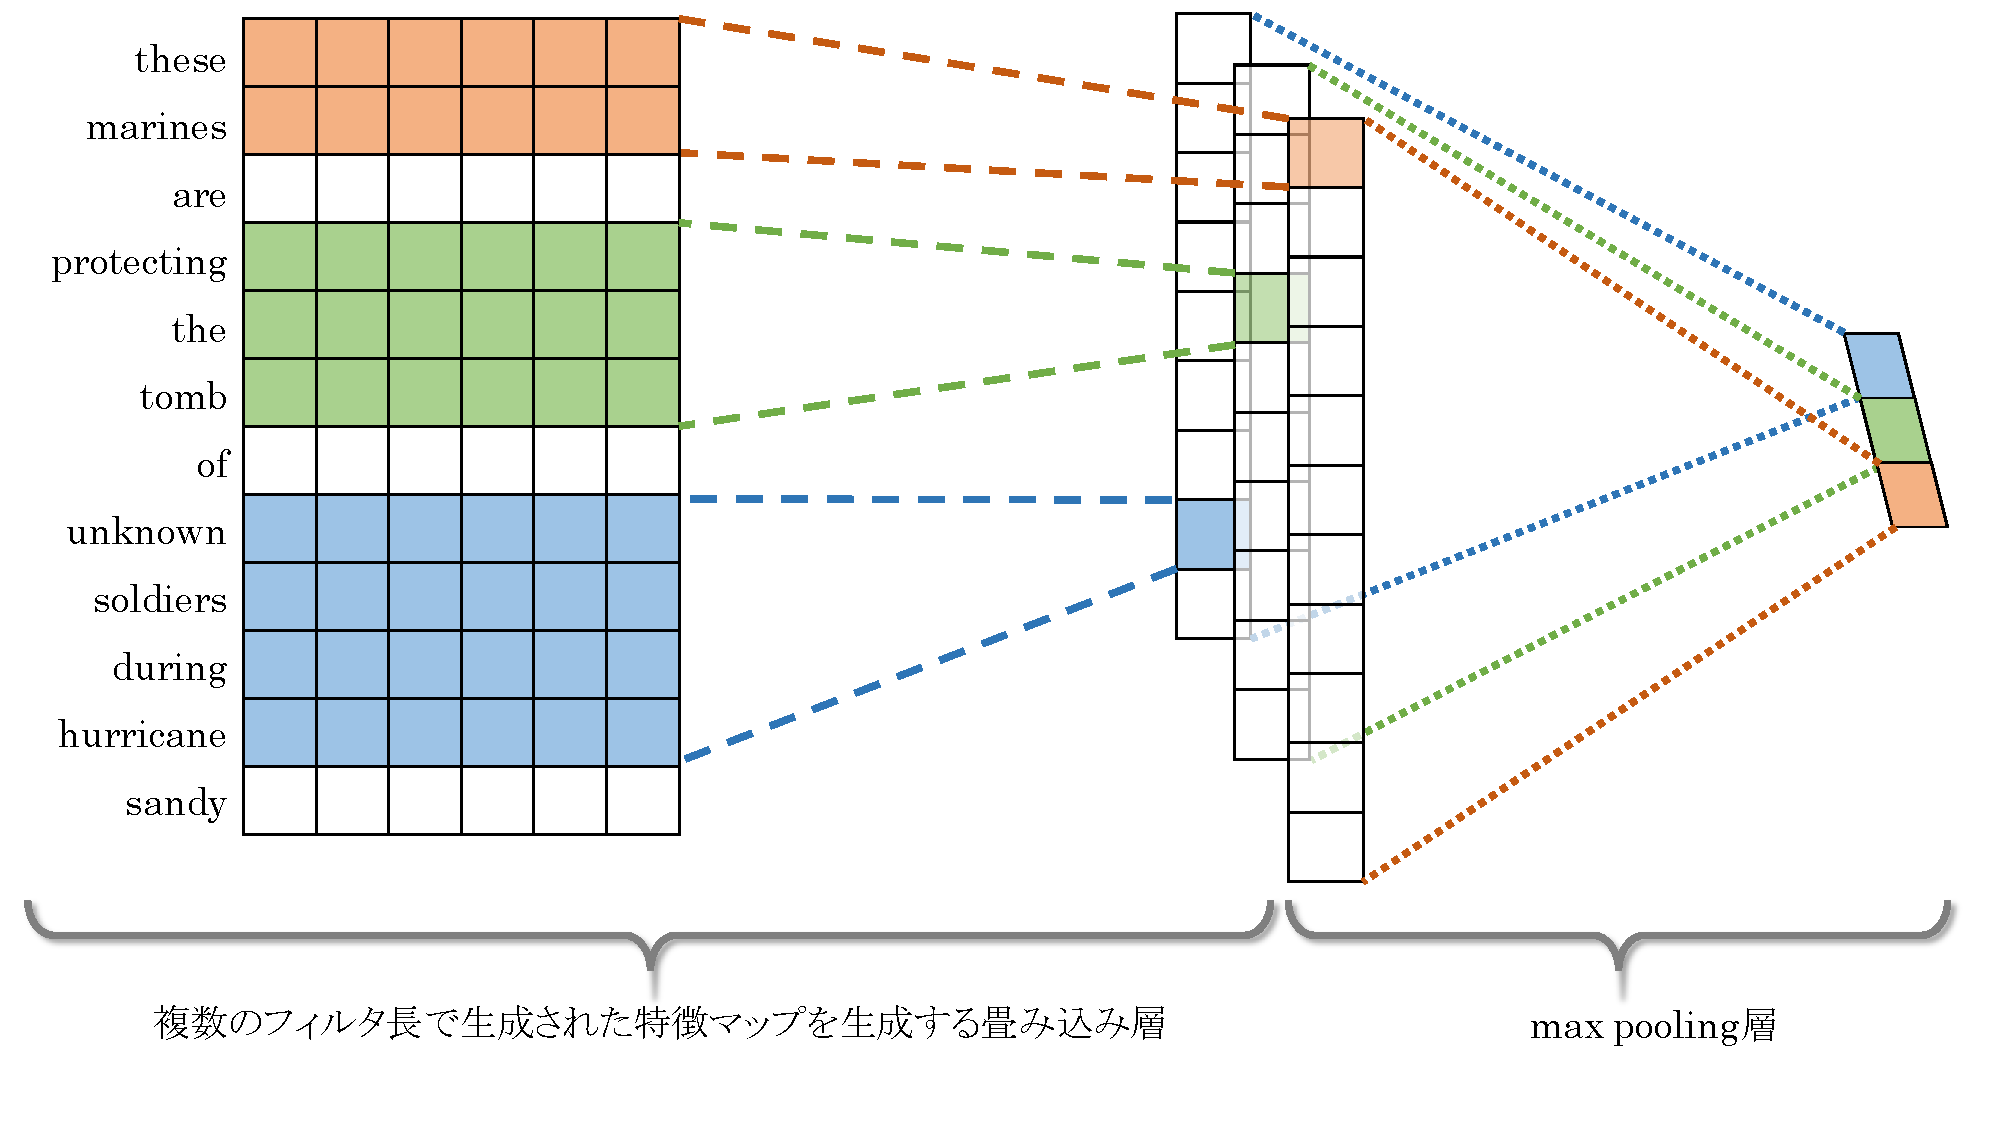
\includegraphics[width=\linewidth]{images/text-cnn.pdf}
    \caption{テキストCNNの図.Wangらの研究\cite{Wang:2018:EEA:3219819.3219903}を参考に作成.}
    \label{fig:text-cnn}
\end{figure}

具体的な手法では,EANNが採用したテキストCNN同じ流れを汲み\cite{Wang:2018:EEA:3219819.3219903},
最終の全結合層の隠れ層に独自にdropoutを採用した形をとった.
dropoutはHintonらによって提案された手法\cite{JMLR:v15:srivastava14a}で,
学習時に指定された確率で無作為に$W_{tf}$内の要素を無効化(0に)してモデルの自由度を制限することで,
モデルが訓練データセットに特化しすぎて汎用性が失われる過学習に繋がりにくくなる利点が報告されたものであった.
%
\subsection{画像特徴}
画像から効率的に特徴を抽出するために,当研究では事前学習済みのVGG19\cite{DBLP:journals/corr/SimonyanZ14a}を起用した.
VGG19は畳み込み16層と全結合層3層から形成され,最終的には1000次元の特徴ベクトルが出力される.
当研究では最終の全結合層のみ改変し,文章特徴のベクトル次元数と同じ数の次元をもつベクトルを出力されるようにした.
また改変した最終全結合層以外は,過学習を防ぐために事前学習の状態を維持することにした.

こうして文章特徴・画像特徴が抽出され,最終的には2つの特徴ベクトルを1つに連結したものが複合特徴である.
連結された複合特徴は,次元数が文章・画像特徴の次元数を足した数となる.
%
\section{ニュース分類器}
%
複合特徴はニュース分類器(図\ref{fig:model}内`pred-fc'が該当)にて正しいニュース・フェイクニュース・ジョークニュースとして分類された.
具体的には隠れ層を含む全結合層とsoftmaxから形成され,最終的な分類が行われた.
モデルの目的は自動で正確に正しいニュース・フェイクニュース・ジョークニュースを分類することである.
そのため正解ラベルを使用して,クロスエントロピー誤差を損失として算出する.
このあと,当研究がベースとしたWangらの研究では確率的勾配降下法(SGD: Stochastic Gradient Descent)
によってパラメータを更新していたが,
当研究では2015年にDiederik P. Kingmaらが提唱したAdamという手法\cite{DBLP:journals/corr/KingmaB14}
を用いてパラメータを更新することにした.
%


%
\chapter{評価実験}
%
\section{データセット}
今回の実験での訓練データセットでは,
Boididouらの研究\cite{boididou2015verifying}によって提案されたTwitter投稿データセットを使用した.
こちらもTwitter上でフェイクニュースを検出するために作られたデータセットであるが,
付加されたラベルとしてReal, Fake, そしてHumorがあり,
ジョークニュースを含めた3カテゴリ分類に適したものとなっているため,当研究で採用した.
データセットでは訓練用と検証用として2部に分かれていたが,
当研究では訓練用とされた部分を対象に10分割交差検定することにした.
データセット内ではツイート文章と画像のみならず,
タイムスタンプや投稿者といったソーシャルコンテキスト情報も含まれている.
当研究ではソーシャルコンテキストは対象に含まず,文章と画像のみで3カテゴリ分類することを目指した.
% 
\section{比較対象手法}
今回,画像つき文章投稿を3カテゴリに分類する提案手法の有効性を調べるために2種類の比較対象手法を用意した.
1つは文章のみで投稿を分類する手法(以降,Textと表記),もう1つは画像のみで投稿を分類する手法(以降,Imageと表記)であった.
いずれも上記提案モデルから文章・画像特徴抽出器を除外したモデルを使用した.
またTextは入力データを提案モデルが使用したデータセットから画像を削除したものを使用した.
Imageは全投稿で使用された画像を対象とし,同じ画像に対して複数の文章投稿があった場合は1件として数えることにした.
% 
\section{実験条件}
%
\subsection{モデル条件}
\subsubsection{Text}
モデルに入力する前に,単語埋め込みへの変換の事前処理として,スムーズに単語埋め込みに変換できるようにするために,
投稿からハッシュタグ(\#)のような記号を除去し,全ての大文字を小文字に変換してスペースで分割した.
投稿から分割された各単語を単語埋め込みに変換する際は,
Google Newsデータセットから事前学習済みのword2vecモデル\cite{google_2013}を使用した.
このモデルでは,各単語を300次元のベクトルに変換するものであった.
ここでwod2vecモデルに該当しない単語が出現した場合,\texttt{<unknown>}としてseed値固定ランダムベクトルを生成することにした.
また,投稿の全単語中50\%以上が\texttt{<unknown>}の場合,実態に則さない学習を避けるために学習対象から外すことにした.
その後テキストCNNに送られ,1つの文章に対して1つの300次元の特徴ベクトルが抽出され,ニュース分類器に渡す形となった.
なお,ウィンドウサイズは2-5までの4種類を用意し,全結合層の隠れ層は1つ用意し,ユニット数は300とした.
隠れ層では50\%のユニットが無視されるDropoutを導入した.
ニュース分類器内でも隠れ層は1つ用意し,ユニット数は300,上記と同じ条件のDropoutも導入した.
%
\subsubsection{Image}
モデルの複雑化を避けるため,1つの投稿に複数枚画像が付加されていた場合は最初の1枚のみをモデルに入力させることにした.
画像は事前学習済みVGG19モデルに入力し,1つの画像に対して1つの300次元のベクトルが抽出され,ニュース分類器に渡す形となった.
本来のVGG19は最終層にて1000次元のベクトルが出力されるが,最終層のみ改変して300次元のベクトルが出力されるようにした.
また前記の通り過学習を避けるために最終層を除き事前学習済みの状態を維持させることにした.
ニュース分類器の条件は上記Textと同一であった.
%
\subsubsection{提案手法}
提案手法では,TextとImageを統合した形をとったため,画像・文章の部分は上記と同様の条件をとった.
画像・文章の特徴を結合するため,ニュース分類器に渡されるのは600次元のベクトルであった.
それにあわせ,隠れ層のユニット数も600とした.
%
\subsection{使用データ統計}
上記の条件を踏まえ,提案手法・Text・Imageが扱う3カテゴリの投稿件数は以下の表\ref{table:posts}の通りである.
Textが使用するデータは提案手法が扱うデータから画像を削除したものであるため,提案手法と全く同じ件数になった.
Imageは,同じ画像に対して複数の投稿があったため,他2手法と比べて非常に少なくなっている.

\begin{table}[h]
    \caption{提案手法と比較対象手法が扱うカテゴリ毎の投稿数}
    \label{table:posts}
    \centering
    \begin{tabular}{clll}
        \hline
        手法 & Real & Fake & Humor \\
        \hline \hline
        Text & 3021 & 4233 & 1509 \\
        Image & 172 & 157 & 82 \\
        提案手法 & 3021 & 4233 & 1509 \\
        \hline
    \end{tabular}
\end{table}

\subsection{評価指標}
評価指標では,Precision(精度), Recall(再現率), F値(左2値の調和平均)を使用することにした.
算出する方法上各カテゴリ毎に上記指標があるが,今回使用するデータセットでは極端にカテゴリが偏っていないので,
各カテゴリの指標を先に算出してから3カテゴリの平均をとるマクロ平均を評価に使うことにした.

\section{実験結果}
3モデルに対して10分割交差検定を行った結果が以下の表\ref{table:result}の通りである.
% 
\begin{table}[h]
    \caption{各モデルの分類成果(マクロ平均)}
    \label{table:result}
    \centering
    \begin{tabular}{clll}
        \hline
        手法 & Precision & Recall & F値 \\
        \hline \hline
        Text & 0.3649 & 0.3677 & 0.3016 \\
        Image & 0.4942 & 0.5055 & 0.4667 \\
        提案手法 & 0.9268 & 0.9362 & 0.9286 \\
        \hline
    \end{tabular}
\end{table}

この結果を見ると,提案手法が他2手法と比べて非常に高い分類成果を挙げたことが読み取れた.
また,比較対象手法内で比べると画像単体の方が分類成果が良好である点もみられた.

\chapter{評価}\label{ch:evaluate}

\section{考察}
今回の評価実験では,提案手法が3指標全てにおいて比較対象手法より優れた分類成績を収めた.
これにより,SNS上で画像つきの投稿を対象にした場合,正しいニュース・フェイクニュースの分類タスクのみならず,
ジョークニュースも含めた分類においても従来のマルチメディア手法のアプローチが有効であることが示唆されたのではないかと考えられる.

また比較対象手法に限って結果を観察すると,文章単体より画像単体の分類の方が優秀な分類成績であった.
これは自然言語より画像の方が分類タスクにおいて研究が進んでいることや,
SNS上の投稿であった故に単語埋め込みに変換する際に\texttt{<unknown>}に変換されやすい傾向にあったことや,
文章の場合英語以外の投稿に対応できないものの,画像においては英語圏以外の投稿であっても十分言語の違いに影響されにくかったことなど,
いくつかの原因が推察される.

提案手法AとBを比較すると,3指標において明確な差はみられなかった.
この点より画像つき投稿を3カテゴリ分類するタスクにおいて,
細かい手法問わず文章・画像それぞれを特徴化・結合して分類することが有効であることが示された.

また表\ref{table:detail}の各カテゴリ毎の成績を見ると,更に興味深い点がいくつか見えてくる.

例えばJokeの分類成績が全手法において一貫してReal\&Fakeより劣悪なものとなった.
これは3カテゴリ内でJokeが最も正しく分類することが困難であることを示唆している.

Textの結果に目を向ける.先述の通りJokeのRecallが0.03と極端に低い結果となり,Real\&FakeのPrecisionが同じく0.52であった.
このことからTextでは正解がJokeである投稿の大多数を見抜くことができず,一部は誤ってFakeと扱われていた可能性が示された.

\section{課題}
今回分類するにあたり,大きな課題となったのが文章投稿の単語埋め込みへの変換であった.
例えば今回使用したデータセットがTwitterから収集されたものであったため,
事前学習済みword2vec手法が対応できない短縮語や造語(ハッシュタグなど)といったユーザ生成コンテンツに対応することが難しかった.

また,この手法に限らずフェイクニュース検出というタスクにおいては,Wangらの研究\cite{Wang:2018:EEA:3219819.3219903}によってある問題点が指摘されていた.
訓練に使ったデータセットが扱うイベントや出来事の特殊性の影響を受けることにより,
検証する時に訓練になかった別のイベントや出来事が使われた場合に正常な判断ができなくなる点であった.

さらに,この手法は英語のみを対象としたものであった点も挙げられた.
データセット内一部では他国の言語が含まれていたため,単語埋め込みに変換する際に大幅に\texttt{<unknown>}に変換される傾向もあった.
%
%
\chapter{おわりに}
%
\section{本論文のまとめ}
本研究では,SNS上で画像と文章を併せて発信された情報に対して,正しいニュース・フェイクニュース・ジョークニュースを判断するモデルを提案した.
実際に3カテゴリ分類を行った結果,文章・画像単体から分類した場合に比べて,全ての評価指標において非常に優秀な分類成績を挙げた.
これによりSNS上における画像つき投稿に対して,ジョークニュースを含めた3カテゴリ分類も有効であることが示された.
%
\section{今後の展望}
このモデルの発展形として,いくつかの方法が考えられる.

例えば文章特徴生成器に対して,テキストCNNではなくVosoughiらの研究\cite{Vosoughi:2016:TLT:2911451.2914762}によってSNS投稿を分析するために提案された,
文字単位でベクトル変換する方法を採用することなどが考えられる.

また,データセットが扱う出来事やイベントによる特殊性の対策として,
Wangらの研究\cite{Wang:2018:EEA:3219819.3219903}では敵対的生成ネットワーク(GAN)を模倣する形をとることが挙げられていた.
このイベントや出来事による特殊性を排するために,真偽分類に加えて扱われたイベントも分類することによって,
特徴化する際に特殊性を排し,フェイクニュースの普遍的な特徴を抽出するようなアプローチが行われていた.
実際にこれによって分類精度が改善した点が上記研究によって報告されていたため,当研究でも有効に働く可能性がある.

提案手法を日本語投稿に対応させることを考えた場合,
まずSNS上で日本語による画像つきの3カテゴリの投稿を収集する必要があると考えられる.
もしも既に日本語投稿による3カテゴリ分類済みのデータセットがあれば投稿を収集する必要はないが,
残念ながら国内に今回使用したデータセットに近い規模をもつものがないのが現状である.

% 

%謝辞
\chapter*{謝辞}
\addcontentsline{toc}{chapter}{謝辞}
本研究を行うにあたり,ご多忙の中,終始適切かつ丁寧なご指導をして下さった大須賀昭彦教授,田原康之准教授,清雄一准教授に深く感謝致します.貴重な勉学の機会を与えてくださったことに深く御礼申し上げます.

%また,研究の機会と議論・研鑽の場を提供して頂き,ご指導頂いた国立情報学研究所/東京大学の本位田真一教授をはじめ活発な議論と貴重なご意見を頂いた研究グループの皆様,大須賀・田原研究室の皆様に感謝の意を表します.さらに,本研究を行う上で必要な楽天公開データの提供に協力してくださいました国立情報学研究所,楽天株式会社の関係者の皆様に感謝の意を表します.

%\chapter*{研究業績}
%\addcontentsline{toc}{chapter}{研究業績}

%\section*{国際会議}
%\begin{achievement}
%\item \underline{\textbf{Minato Sato}}, Ryohei Orihara, Sei Yuichi, Yasuyuki Tahara and Akihiko Ohsuga: Japanese Text Classification by Character-Level Deep ConvNets and Transfer Learning, The 9th International Coneference on Agents and Artificial Intelligence (ICAART2017), Feb 2017. (accepted as a Full Paper)
%\end{achievement}

%\section*{査読付き国内シンポジウム・ワークショップ}
%\begin{achievement}
%\item \underline{\textbf{佐藤挙斗}},折原良平,清雄一,田原康之,大須賀昭彦: 文字レベル深層学習による日本語テキストの分類と転移学習,合同エージェントワークショップ&シンポジウム2016 (JAWS2016),pp.199-206,2016年9月. (ショート発表) \textcolor{red}{{\bf 優秀発表賞}}
%\end{achievement}

%\section*{研究会}
%\begin{achievement}
%\item \underline{\textbf{佐藤挙斗}},折原良平,清雄一,田原康之,大須賀昭彦: 文字レベル深層学習の日本語データセットへの応用,第184回 情報処理学会 知能システム研究会 (SIG-ICS) ,2016年8月.
%\item \underline{\textbf{佐藤挙斗}},折原良平,清雄一,田原康之,大須賀昭彦: 文字レベル深層学習によるテキスト分類と転移学習,人工知能学会 第102回人工知能基本問題研究会(SIG-FPAI),2016年12月. 
%\end{achievement}

%参考文献
\newpage
% \bibliographystyle{plain}
% \bibliography{./tex/ref/ref}
%\bibliography{reference_slim}
%\bibliographystyle{plain}

\begin{thebibliography} {*}
%\bibitem{sibata} 柴田雅博,冨浦洋一,西口友美, 
%\textit{雑談自由対話を実現するためのWWW 上の文書からの妥当な候補文選択手法}
%	,人工知能学会論文誌,vol.24, no.6, pp.507-519, 2009.

%\bibitem{sugeo} LeFevre, K., DeWitt, D. and Ramakrishnan, R., 
%\textit{Mondrian Multidimensional K - Anonymity}
%	, Proc. IEEE ICDE, pp. 25 - 25, 2006.

\end{thebibliography}

%付録
%%
\appendix
\renewcommand{\thesection}{付録.\ \arabic{section}}
\renewcommand{\thesubsection}{\ \arabic{section}-\arabic{subsection}}
%
\section{統計表3  推計患者数,年齢階級・傷病大分類別}
\subsection{分類表1}
%
\begin{figure}[h]
  \begin{center}
    \includegraphics[width=\fullwidth]{./img/図1.jpg}
    %\caption{傷病大分類1}
  \end{center}
\end{figure}
%
\newpage
\subsection{分類表2}
%
\begin{figure}[h]
  \begin{center}
    \includegraphics[width=\fullwidth]{./img/図2.jpg}
    %\caption{傷病大分類2}
  \end{center}
\end{figure}
%
\newpage
\section{統計表9  総患者数,性・主な傷病別 }
%
\begin{figure}[h]
  \begin{center}
    \includegraphics[width=0.8\fullwidth]{./img/図3.jpg}
    %\caption{傷病大分類3}
  \end{center}
\end{figure}


%

\newpage
\printindex
%
%
\end{document}